\section{Hardware design}

The central unit of the system is the BeagleBone Black single-board computer. This computer produced by Texas Instruments was chosen because it's high performance to cost ratio (important for Python) and it's extensive peripheral support.
The BeagleBone Black (BBB) is shipped with preinstalled Angström Linux, which is a lightweight Linux distribution developed for embedded devices. The advantages of using a linux distribution as an embedded operating system include the easy remote access to the system core via SSH, integrated package manager (opkg) with precompiled software distributions for the system (Python, bluez), and generally high community support.

The BBB doesn't contain any integrated sensors, but can be extended with Capes, specialized for different tasks. As the BMESHIP is in a prototype stage, only the most essential sensors will be installed, without the assistance of Capes.

The system contains only a small amount of electronics, assembled on a breadboard. The power to the BeagleBone is supplied from the 12V battery by a 5V voltage regulator IC through USB Cable.
Unfortunately the BeagleBone shuts down the USB devices if it’s powered through the regular 2.1 / 5.5 mm power cable, therefore we “trick” the device into thinking that it’s supplied from a regular usb device.

\begin{figure}[H]
	\centering
	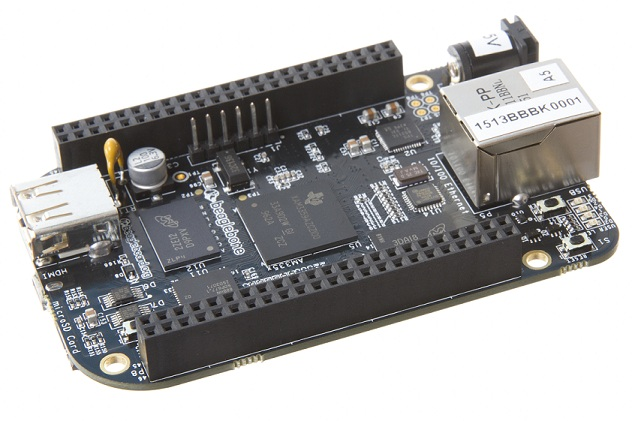
\includegraphics[width=0.7\textwidth]{img2/BeagleBone}
	\caption{The physical layout of the system}
	\label{fig:PhysicalLayout}
\end{figure}

Additional electronics include the motor controller board and the servo control, but unfortunately not all of the required parts are available yet.

\subsection{Remote control}

The Man-in-the-loop operation mode has been realized using a commercial two-channel 2.4GHz RC transmitter and receiver. CH1 is responsible for the throttle, or rig control, while CH2 controls the course through the rudder. The output of both channels are standard servo signals.

\begin{figure}[H]
	\centering
	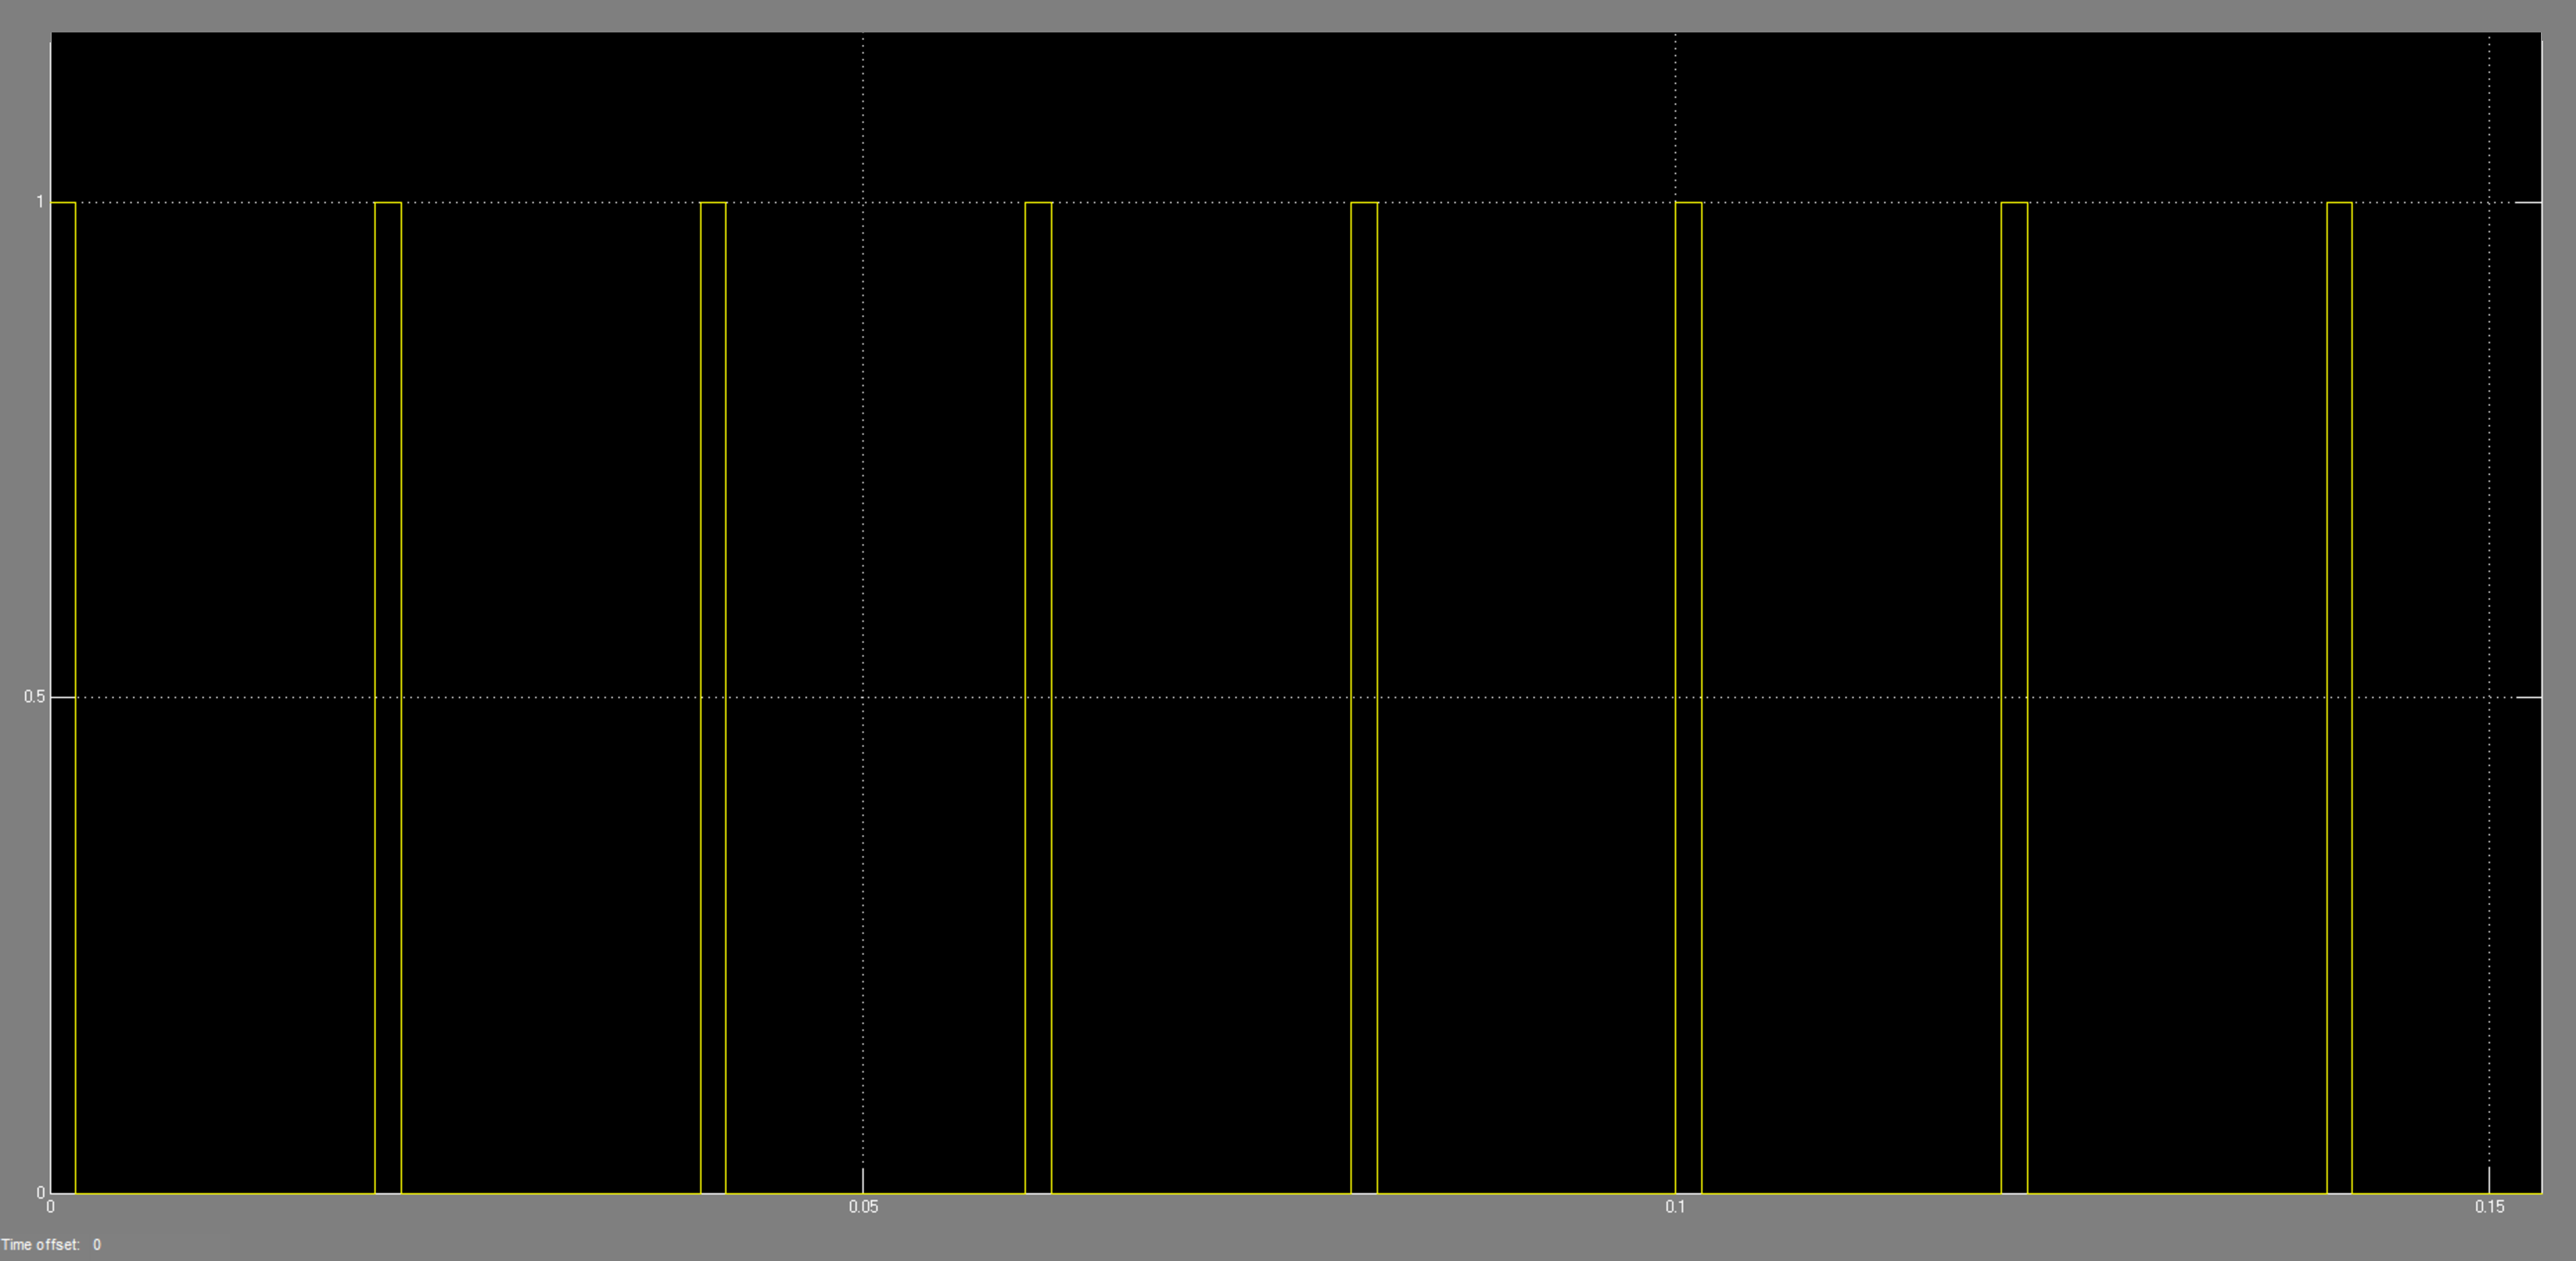
\includegraphics[width=0.7\textwidth]{fig/servosignal}
	\caption{Servo signal form}
	\label{fig:Servosignal}
\end{figure}

\subsection{Wind sensor}

In order to effectively control a sailing ship, the wind direction must be determined with sufficient precision relative to the body of the ship. Note that sufficient in this context means a generally low precision requirement, but the availability and reliability of that measurement is critical. Several different methods of detection have been investigated:

\paragraph{Incremental encoder} Detection is possible using incremental encoders, and a very high angle precision can be assured. However, in case of a system error or restart, the encoder must be re-calibrated to rely on it again. In addition, some amount of missed signals is inevitable, which would introduce an absolute error to the measurement that can't be neglected.

Advantages:
\begin{itemize}
\item Low cost
\item Very high precision
\item Quick response
\end{itemize}

Disadvantages:
\begin{itemize}
\item On-site hardware processing required
\item Requires frequent recalibration
\item Requires external recalibration hardware
\end{itemize}


Of course an absolute angle encoder is immune to these problems. An enclosed system is capable of providing precise, reliable and always available data about the wind direction. Alas, the price range of the cheapest of these sensors is way out of the scope of the current project.

Advantages:
\begin{itemize}
\item High precision
\item Quick response
\item Always available, reliable
\end{itemize}

Disadvantages:
\begin{itemize}
\item Very-very expensive
\end{itemize}


A slightly different approach is to use a multiturn potentiometer and estimate the angle position using an Analog to Digital Converter. Though unfortunately such multiturn potentiometers are unable to perform arbitrary number of rotations in the same direction, therefore their ability is limited.

Advantages:
\begin{itemize}
\item Low cost
\item Easy to process
\item sufficient precision
\end{itemize}

Disadvantages:
\begin{itemize}
\item Can't rotate infinitely
\end{itemize}


There's a somewhat similar approach that consists of a permanent magnet and a number of analog magnetic field sensors. Either the magnet or the Hall effect sensors are attached to the rotating wind-indicator, while the other part remains fixed to the ship. Processing the signals of 2 (or 4 to compensate for noise) sensors with an ADC and applying adequate trigonometrical processing on the raw data results in an absolute wind direction measurement. Though the required sensor post-processing is heavy on a smaller microcontroller, because of the required inverse trigonometrical functions, this is hardly a factor on a single board computer like the BeagleBone.

Advantages:
\begin{itemize}
\item Low cost
\item Sufficient precision
\item Absolute, reliable
\end{itemize}

Disadvantages:
\begin{itemize}
\item Complex software post-processing required
\item Susceptible to noise
\end{itemize}


After carefully considering the possibilities, the Magnet-based wind detection was chosen. Optionally a wind speed detector can be assembled using incremental encoders.

[img and schematic of the sensor]

\subsection{Hardware}

\subsection{Assembly}